%	http://www.texample.net/tikz/examples/focused-ion-beam-system/
\documentclass[tikz]{standalone}
\usetikzlibrary{arrows,decorations.pathmorphing}
\def\english#1{\emph{#1}}
\tikzset{
  arrow/.style={-stealth', line width=0.5pt},
  every picture/.append style={line width=1pt},
}
\begin{document}
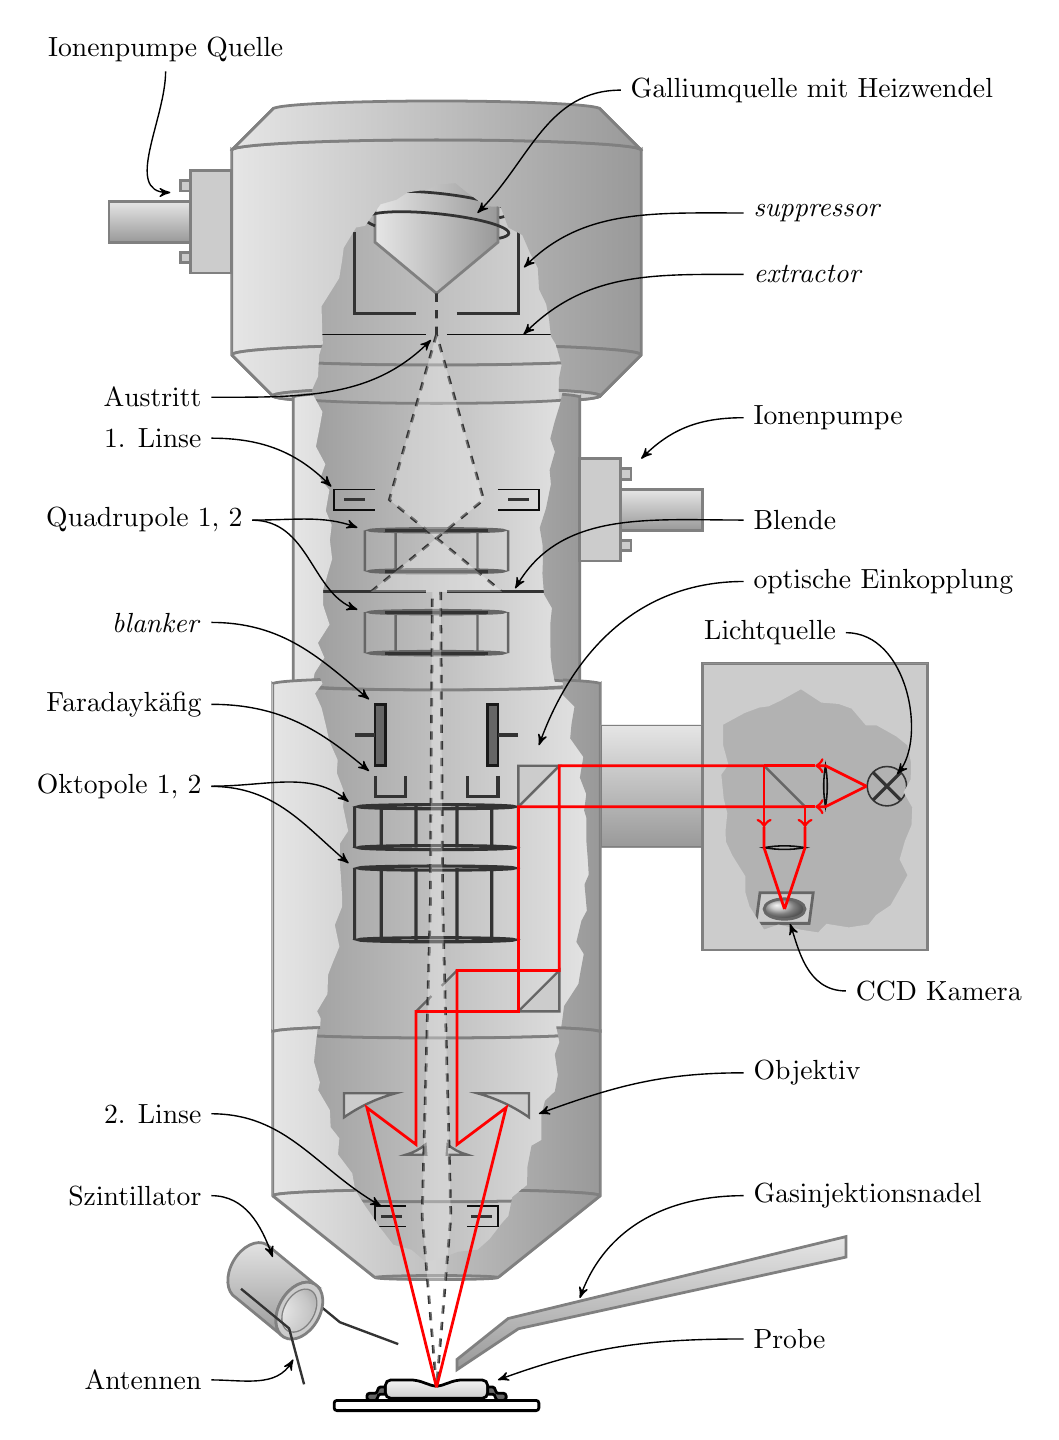
\begin{tikzpicture}[
    scale=1.3,
    fib housing horz/.style={top color=black!10, bottom color=black!40, draw=black!50},
    fib housing vert/.style={left color=black!10, right color=black!40, draw=black!50},
    fib housing/.style={fill=black!20, draw=black!50},
    fib background vert/.style={left color=black!40, right color=black!10, draw=black!50},
    fib background/.style={fill=black!30, draw=black!50},
    fib lens thick/.style={draw=black!80, line width=0.04cm},
    fib lens thinn/.style={draw=black!95, line width=0.02cm},
    fib mirror/.style={draw=black!60, line width=0.03cm, fill=black!20},
    fib objective/.style={draw=black!60, line width=0.03cm},
    fib quadrupole/.style={draw=black!60, line width=0.03cm},
    fib blanker/.style={draw=black!90, fill=black!60},
    fib octopole/.style={draw=black!80, line width=0.04cm},
  ]
  % Picture created and copyright by Clemens Helfmeier in 2009 for master thesis.
  % Contact me at: Clemens@Helfmeier.de
  % Aufbau des FIBs
  % "falsch" herum, Probe unten, Ionen oben
  % einzelne Elemente sind rund, insofern auch shading anbringen
  % jedes element ist 1.4cm hoch.
  % Die FIB-Säule
  \begin{scope}[scale=2]
    \begin{scope}[yshift=0.2]
      %% Ionenquelle
      { % Rückseite
        \path[fib background vert]
          (-1,0) arc (180:360:1 and 0.05) -- (1,-1) arc (360:180:1 and 0.05) --cycle;
        \path[fib background vert]
          (-0.8,0.2) arc (180:360:0.8 and 0.04) -- (1,0) arc (360:180:1 and 0.05) --cycle;
        \path[fib background vert]
          (-0.8,-1.2) arc (180:360:0.8 and 0.04) -- (1,-1) arc (360:180:1 and 0.05) --cycle;
      }
      { % Innenleben
        \path[fib housing vert]
          (-0.3,0) -- (0.3,0) -- (0.3,-0.45) -- (0,-0.7) coordinate (source) -- (-0.3,-0.45) --cycle;
        \path[draw=black!80, yslant=-0.1]
          \foreach \x in {0.1,0.2,0.3,0.4} {
            (-0.3,-\x) arc(210:-30:0.35 and 0.06)
          };
        \path[fib lens thinn]
          (-0.8,-0.9) -- (-0.05,-0.9)
          (0,-0.9) coordinate (emitter)
          (0.05,-0.9) -- (0.8,-0.9) coordinate[midway] (extractor);
        \path[fib lens thick]
          (-0.4,-0.4) -- (-0.4,-0.8) -- (-0.1,-0.8) (0.1,-0.8) -- (0.4,-0.8) -- (0.4,-0.4) coordinate[midway] (suppressor);
      }
      \begin{scope} % Gehäuse
        \path[clip,decoration={random steps, segment length=6pt, amplitude=2pt}]
          (-1,0.3) -- (1,0.3) -- (1,-1.3)
          -- (0.6,-1.3) decorate{ ..controls (0.6,0.2) and (-0.6,0.2).. (-0.6,-1.3)}
          -- (-1,-1.3) --cycle;
        \path[fib housing vert]
          (-1,0) arc (180:0:1 and 0.05) -- (1,-1) arc (0:180:1 and 0.05) --cycle;
        \path[fib housing vert]
          (-0.8,0.2) arc (180:0:0.8 and 0.04) -- (1,0) arc (0:180:1 and 0.05) --cycle;
        \path[fib housing vert]
          (-0.8,-1.2) arc (180:0:0.8 and 0.04) -- (1,-1) arc (0:180:1 and 0.05) --cycle;
        \path[fib housing]
          (0,-1.2) ellipse (0.8 and 0.04);
      \end{scope}
      { % Ionenpumpe extern
        \path[fib housing]
          (-1,-0.1) rectangle (-1.2,-0.6);
        \path[fib housing]
          (-1.2,-0.15) rectangle (-1.25,-0.2)
          (-1.2,-0.55) rectangle (-1.25,-0.5);
        \path[fib housing horz]
          (-1.2,-0.25) rectangle (-1.6,-0.45);
      }
    \end{scope}
    %% Beschleunigung und fokussierung
    \begin{scope}[yshift=-1.4cm]
      { % Rückseite
        \path[fib background vert]
          (-0.7,0.2) arc (180:360:0.7 and 0.03) -- (0.7,-1.2) arc (360:180:0.7 and 0.03) --cycle;
      }
      { % Innenleben
        \path[fib lens thinn] % Linse
          (-0.3,-0.25) -- (-0.5,-0.25) -- (-0.5,-0.35) -- (-0.3,-0.35)
          (0.3,-0.25) -- (0.5,-0.25) -- (0.5,-0.35) -- (0.3,-0.35);
        \path[fib lens thick]
          (-0.45,-0.3) -- (-0.35,-0.3) (0.35,-0.3) -- (0.45,-0.3)
          (0,-0.3) coordinate (ionlens1)
          (-0.5,-0.25) coordinate (linse1);
        \path[fib quadrupole] % quadrupole 1
          (0,-0.45) ellipse (0.33cm and 0.01cm)
          (0,-0.65) ellipse (0.33cm and 0.01cm)
          (-0.35,-0.45) -- ++(0,-0.2) (-0.2,-0.45) -- ++(0,-0.2)
          (0.35,-0.45) -- ++(0,-0.2) (0.2,-0.45) -- ++(0,-0.2)
          (-0.35,-0.45) coordinate (quadA);
        \path[fib lens thick]
          (-0.25,-0.45) -- (0.25,-0.45)
          (-0.25,-0.65) -- (0.25,-0.65);
        \path[fib lens thick] % Blende
          (-0.7,-0.75) -- (-0.05,-0.75) (0.05,-0.75) -- (0.7,-0.75) coordinate[midway] (blende)
          (0,-0.75) coordinate (ionblende);
        \path[fib quadrupole] % quadrupole 2
          (0,-0.85) ellipse (0.33cm and 0.01cm)
          (0,-1.05) ellipse (0.33cm and 0.01cm)
          (-0.35,-0.85) -- ++(0,-0.2) (-0.2,-0.85) -- ++(0,-0.2)
          (0.35,-0.85) -- ++(0,-0.2) (0.2,-0.85) -- ++(0,-0.2)
          (-0.35,-0.85) coordinate (quadB);
        \path[fib lens thick]
          (-0.25,-0.85) -- (0.25,-0.85)
          (-0.25,-1.05) -- (0.25,-1.05);
      }
      \begin{scope} % Gehäuse
        \path[clip,decoration={random steps, segment length=6pt, amplitude=2pt}]
          (0.7,0.3) -- (0.7,-1.3)
          -- (0.6,-1.3) decorate{ ..controls (0.5,-0.6).. (0.6,0.3)} --cycle
          (-0.7,0.3) -- (-0.6,0.3) decorate{ ..controls (-0.5,-0.6).. (-0.6,-1.3)}
          -- (-0.7,-1.3) --cycle;
        \path[fib housing vert]
          (-0.7,0.2) arc (180:0:0.7 and 0.03) -- (0.7,-1.2) arc (0:180:0.7 and 0.03) --cycle;
      \end{scope}
      { % Ionenpumpe extern
        \path[fib housing]
          (0.7,-0.1) rectangle (0.9,-0.6);
        \path[fib housing]
          (0.9,-0.15) rectangle (0.95,-0.2) (0.95,-0.15) coordinate (ionenpume)
          (0.9,-0.55) rectangle (0.95,-0.5);
        \path[fib housing horz]
          (0.9,-0.25) rectangle (1.3,-0.45);
      }
    \end{scope}
    \begin{scope}[yshift=-2.8cm]
      % Optik und Ablenkteile
      { %Rückseite
        \path[fib background vert]
          (-0.8,0.2) arc (180:360:0.8 and 0.03) -- (0.8,-1.5) arc (360:180:0.8 and 0.03) --cycle;
        \path[fib background]
          (1.3,0.3) rectangle (2.4,-1.1);
      }
      { % Innenleben
        \path[fib blanker] % blanker
          (-0.3,0.1) rectangle (-0.25,-0.2)
          (0.3,0.1) rectangle (0.25,-0.2)
          (-0.3,0.1) coordinate (blanker);
        \path[fib lens thick]
          (-0.3,-0.05) -- (-0.4,-0.05) (0.3,-0.05) -- (0.4,-0.05);
        \path[fib lens thick] % Faradaykäfig
          (-0.3,-0.25) -- (-0.3,-0.35) -- (-0.15,-0.35) -- (-0.15,-0.25)
          (-0.3,-0.25) coordinate (faraday)
          (0.3,-0.25) -- (0.3,-0.35) -- (0.15,-0.35) -- (0.15,-0.25);
        \path[fib octopole] % octopole 1
          (0,-0.4) ellipse (0.38cm and 0.01cm)
          (0,-0.6) ellipse (0.38cm and 0.01cm)
          (-0.4,-0.4) -- (-0.4,-0.6) (0.4,-0.4) -- (0.4,-0.6)
          (-0.27,-0.4) -- ++(0,-0.2) (-0.1,-0.4) -- ++(0,-0.2)
          (0.27,-0.4) -- ++(0,-0.2) (0.1,-0.4) -- ++(0,-0.2)
          (0,-0.5) coordinate (ionocto1)
          (-0.4,-0.4) coordinate (octoA);
        \path[fib octopole] % octopole 2
          (0,-0.7) ellipse (0.38cm and 0.01cm)
          (0,-1.05) ellipse (0.38cm and 0.01cm)
          (-0.4,-0.7) -- (-0.4,-1.05) (0.4,-0.7) -- (0.4,-1.05)
          (-0.27,-0.7) -- ++(0,-0.35) (-0.1,-0.7) -- ++(0,-0.35)
          (0.27,-0.7) -- ++(0,-0.35) (0.1,-0.7) -- ++(0,-0.35)
          (0,-0.88) coordinate (ionocto2)
          (-0.4,-0.7) coordinate (octoB);
        \path[fib mirror]
          (0.4,-0.4) -- (0.6,-0.2) -- (0.4,-0.2) -- cycle;
        \path[fib mirror]
          (0.6,-1.2) -- (0.4,-1.4) -- (0.6,-1.4) -- cycle;
        \path[fib mirror]
          (-0.1,-1.4) -- (-0.025,-1.325) (0.025,-1.275) -- (0.1,-1.2) -- cycle;
        \path[fib mirror] % kamera innenleben
          (1.6,-0.2) -- (1.8,-0.4);
        \path[fib lens thinn]
          (1.6,-0.6) arc(100:80:0.575) arc(-80:-100:0.575) -- cycle;
        \path[draw=black!60, fill=black!20]
          (1.58,-0.82) -- (1.56,-0.97) -- (1.82,-0.97) -- (1.84,-0.82) --cycle;
        \path[draw=black!60, shading=ball, ball color=black!30]
          (1.7,-0.9) ellipse (0.1cm and 0.05cm);
        \begin{scope}
          \path[clip]
            (2.2,-0.3) circle (0.1cm);
          \path[draw=black!80, line width=0.04cm]
            (2.2,-0.3) circle (0.1cm)
            (2.1,-0.2) -- (2.3,-0.4)
            (2.1,-0.4) -- (2.3,-0.2);
        \end{scope}
        \path[fib lens thinn]
          (1.9,-0.2) arc(170:190:0.575) arc(-10:10:0.575) -- cycle;
      }
      \begin{scope} % externes Gehäuse
        \path[clip,decoration={random steps, segment length=6pt, amplitude=2pt}]
          (0.8,0) -- (1.3,0) -- (1.3,0.3) -- (2.4,0.3) -- (2.4,-1.1) -- (1.3,-1.1) -- (1.3,-0.6) -- (0.8,-0.6) -- (0.8,-0.1) -- (1.4,-0.1)
          decorate{ .. controls (1.4,-0.5) .. (1.6,-1) .. controls (2.3,-1) .. (2.3,-0.1) .. controls (1.8,0.2) .. (1.4,0)}
          -- (1.4,-0.1) -- (0.8,-0.1) --cycle;
        \path[fib housing horz]
          (0.8,0) rectangle (1.3,-0.6);
        \path[fib housing]
          (1.3,0.3) rectangle (2.4,-1.1);
      \end{scope}
      \begin{scope} % Gehäuse
        \path[clip,decoration={random steps, segment length=6pt, amplitude=2pt}]
          (0.8,0.3) -- (0.8,-1.6)
          -- (0.6,-1.6) decorate{ ..controls (0.8,-0.6).. (0.6,0.3)} --cycle
          (-0.8,0.3) -- (-0.6,0.3) decorate{ ..controls (-0.4,-0.6).. (-0.6,-1.6)}
          -- (-0.8,-1.6) --cycle;
        \path[fib housing vert]
          (-0.8,0.2) arc (180:0:0.8 and 0.03) -- (0.8,-1.5) arc (0:180:0.8 and 0.03) --cycle;
      \end{scope}
    \end{scope}
    \begin{scope}[yshift=-4.5cm]
      % Deckel
      { % Rückwand
        \path[fib background vert]
          (-0.8,0.2) arc (180:360:0.8 and 0.03) -- (0.8,-0.6) arc (360:180:0.8 and 0.03) -- cycle;
        \path[fib background vert]
          (0.8,-0.6) arc (360:180:0.8 and 0.03) -- (-0.3,-1) arc (180:360:0.3 and 0.01) -- cycle;
      }
      { % Innenleben
        \path[fib mirror]
          (-0.15,-0.4) arc (-75:-50:0.25) -- (-0.05,-0.4) -- cycle;
        \path[fib mirror]
          (0.15,-0.4) arc (-105:-130:0.25) -- (0.05,-0.4) -- cycle;
        \path[fib mirror]
          (-0.2,-0.1) arc (105:125:0.8) coordinate (tmp) -- (tmp |- -0.2,-0.1) --cycle;
        \path[fib mirror]
          (0.2,-0.1) arc (75:55:0.8) coordinate (tmp) -- (tmp |- 0.2,-0.1) --cycle;
        \path[fib lens thinn] % 2. Linse
          (-0.15,-0.65) -- (-0.3,-0.65) -- (-0.3,-0.75) -- (-0.15,-0.75)
          (0.15,-0.65) -- (0.3,-0.65) -- (0.3,-0.75) -- (0.15,-0.75);
        \path[fib lens thick]
          (-0.27,-0.7) -- (-0.17,-0.7) (0.17,-0.7) -- (0.27,-0.7)
          (0,-0.7) coordinate (ionlens2)
          (-0.27,-0.65) coordinate (linse2);
      }
      \begin{scope} % Gehäuse
        \path[clip,decoration={random steps, segment length=6pt, amplitude=2pt}]
          (-0.8,0.3) -- (-0.6,0.3) decorate{ ..controls (-0.5,-1.3) and (0.5,-1.3).. (0.6,0.3)}
          -- (0.8,0.3) -- (0.8,-1) -- (-0.8,-1) -- cycle;
        \path[fib housing vert]
          (-0.8,0.2) arc (180:0:0.8 and 0.03) -- (0.8,-0.6) arc (0:180:0.8 and 0.03) -- cycle;
        \path[fib housing vert]
          (0.8,-0.6) arc (0:180:0.8 and 0.03) -- (-0.3,-1) arc (180:0:0.3 and 0.01) -- cycle;
      \end{scope}
    \end{scope}
    \begin{scope}[yshift=-6cm, scale=0.5]
      % Probe
      \path[draw, rounded corners=1pt]
        (-1,-0.2) rectangle (1,-0.3);
      \path[draw, fill, top color=black!5, bottom color=black!20, rounded corners=2pt]
        (-0.5,0) -- (-0.5,-0.18) -- (0.5,-0.18) -- (0.5,0) -- (0.2,0) -- (0,-0.07) -- (-0.2,0) -- cycle
        (0,-0.07) coordinate (target);
      \path[draw, fill=black!60]
        (-0.5,-0.07) -- (-0.55,-0.07) to[out=180, in=0] (-0.6,-0.13) {[rounded corners=1pt] -- (-0.68,-0.13) --
          (-0.68,-0.2)} -- (-0.6,-0.2) to[out=0, in=180] (-0.55,-0.14) -- (-0.5,-0.14) -- cycle;
      \path[draw, fill=black!60]
        (0.5,-0.07) -- (0.55,-0.07) to[out=0, in=180] (0.6,-0.13) {[rounded corners=1pt] -- (0.68,-0.13) --
          (0.68,-0.2)} -- (0.6,-0.2) to[out=180, in=0] (0.55,-0.14) -- (0.5,-0.14) -- cycle;
    \end{scope}
    \begin{scope}[yshift=-5.7cm, rotate around={-30:(-0.75,0.2)}]
      % Szintillator
      \path[draw=black!80, line width=0.03cm] % 1. Antenne
        (-0.7,0.2) -- (-0.4,0.15) -- (-0.1,0.2);
      \path[fib housing horz]
        (-0.9,0.3) -- (-0.6,0.25) arc(90:270:0.1 and 0.15) -- (-0.9,0) arc(270:90:0.1 and 0.15) --cycle;
      \path[fib housing]
        (-0.6,0.1) ellipse (0.1 and 0.15);
      \begin{scope}
        \path[fib housing]
          (-0.6,0.1) ellipse (0.07 and 0.11);
        \path[clip]
          (-0.6,0.1) ellipse (0.07 and 0.11);
        \path[shading=ball, ball color=black!30]
          (-0.5,0) circle (0.4);
      \end{scope}
      \path[draw=black!80, line width=0.03cm] % 2. Antenne
        (-0.9,0.05) -- (-0.6,0) -- (-0.4,-0.2);
    \end{scope}
    \begin{scope}[yshift=-6cm]
      % Gasnadel
      \path[fib housing horz]
        (2,0.7) -- (0.35,0.3) -- (0.1,0.1) -- (0.1,0.05) -- (0.4,0.25) -- (2,0.6) -- cycle;
    \end{scope}
    \begin{scope} % Strahlen
      % Ionen
      \path[draw=black!80, dashed]
        (source) -- (emitter)
        (emitter) -- (ionlens1 -| -0.23,0) -- (ionblende -| 0.32,0)
        (ionblende -| 0.02,0) -- (ionocto1 -| 0.028,0) -- (ionocto2 -| 0.03,0) -- (ionlens2 -| 0.07,0) --
        (target) --
        (ionlens2 -| -0.07,0) -- (ionocto2 -| -0.03,0) -- (ionocto1 -| -0.028,0) -- (ionblende -| -0.02,0)
        (ionblende -| -0.32,0) -- (ionlens1 -| 0.23,0) -- (emitter);
      \path[fill=white, opacity=0.3]
        (emitter) -- (ionlens1 -| -0.23,0) -- (ionblende -| 0.32,0) --
        (ionblende -| 0.02,0) -- (ionocto1 -| 0.028,0) -- (ionocto2 -| 0.03,0) -- (ionlens2 -| 0.07,0) --
        (target) --
        (ionlens2 -| -0.07,0) -- (ionocto2 -| -0.03,0) -- (ionocto1 -| -0.028,0) --
        (ionblende -| -0.02,0) -- (ionblende -| -0.32,0) -- (ionlens1 -| 0.23,0) -- cycle;
      % Licht
      \path[draw=red]
        (1.6,-3) -- (0.6,-3) -- (0.6,-4) -- (0.1,-4) -- (0.1,-4.85) -- (0.34,-4.67) -- (target)
        (1.8,-3.2) -- (0.4,-3.2) -- (0.4,-4.2) -- (-0.1,-4.2) -- (-0.1,-4.85) -- (-0.34,-4.67) -- (target);
      \path[draw=red,->]
        (2.1,-3.1) -- (1.9,-3) -- (1.85,-3);
      \path[draw=red,->]
        (2.1,-3.1) -- (1.9,-3.2) -- (1.85,-3.2);
      \path[draw=red]
        (1.85,-3) -- (1.6,-3)
        (1.85,-3.2) -- (1.8,-3.2);
      \path[draw=red,->]
        (1.6,-3) -- (1.6,-3.3);
      \path[draw=red,->]
        (1.8,-3.2) -- (1.8,-3.3);
      \path[draw=red]
        (1.7,-3.7) -- (1.6,-3.4) -- (1.6,-3.3)
        (1.7,-3.7) -- (1.8,-3.4) -- (1.8,-3.3);
    \end{scope}
    % Beschriftung
    \begin{scope}[arrow]
      \path[draw] (0.9,0.3) node[anchor=west] {Galliumquelle mit Heizwendel} to[out=180, in=45] (0.2,-0.3);
      \path[draw] (1.5,-0.6) node[anchor=west] {\english{extractor}} to[out=180, in=45] (extractor);
      \path[draw,shorten >=0.1cm] (1.5,-0.3) node[anchor=west] {\english{suppressor}} to[out=180, in=45] (suppressor);
      \path[draw] (-0.7,0.5) node[anchor=east] (tmp) {Ionenpumpe Quelle} (tmp) to[out=-90, in=180] (-1.3, -0.2);
      \path[draw,shorten >=0.1cm] (-1.1,-1.2) node[anchor=east] {Austritt} to[out=0, in=225] (emitter);
      \path[draw] (1.5,-1.3) node[anchor=west] {Ionenpumpe} to[out=180, in=45] (1,-1.5);
      \path[draw,shorten >=0.1cm] (-0.9,-1.8) node[anchor=east] (quad) {Quadrupole 1, 2} to[out=0, in=160] (quadA);
      \path[draw,shorten >=0.1cm]  (quad) to[out=0, in=160] (quadB);
      \path[draw,shorten >=0.05cm] (-1.1,-1.4) node[anchor=east] {1. Linse} to[out=0, in=135] (linse1);
      \path[draw,shorten >=0.05cm] (1.5,-1.8) node[anchor=west] {Blende} to[out=180, in=60] (blende);
      \path[draw, shorten >=0.1cm] (-1.1,-2.3) node[anchor=east] {\english{blanker}} to[out=0, in=140] (blanker);
      \path[draw, shorten >=0.1cm] (-1.1,-2.7) node[anchor=east] {Faradaykäfig} to[out=0, in=140] (faraday);
      \path[draw, shorten >=0.1cm] (-1.1,-3.1) node[anchor=east] (okto) {Oktopole 1, 2} to[out=0, in=140] (octoA);
      \path[draw, shorten >=0.1cm] (okto) to[out=0, in=140] (octoB);
      \path[draw] (1.5,-2.1) node[anchor=west] {optische Einkopplung} to[out=180, in=70] (0.5, -2.9);
      \path[draw,shorten >=0.2cm] (2,-2.35) node[anchor=east] {Lichtquelle} to[out=0, in=50] (2.2,-3.1);
      \path[draw, shorten >=0.2cm] (2,-4.1) node[anchor=west] {CCD Kamera} to[out=180, in=-70] (1.7,-3.7);
      \path[draw] (1.5,-4.5) node[anchor=west] {Objektiv} to[out=180, in=20] (0.5,-4.7);
      \path[draw] (-1.1,-4.7) node[anchor=east] {2. Linse} to[out=0, in=150] (linse2);
      \path[draw] (1.5,-5.1) node[anchor=west] {Gasinjektionsnadel} to[out=180, in=70] (0.7,-5.6);
      \path[draw] (1.5,-5.8) node[anchor=west] {Probe} to[out=180, in=20] (0.3,-6);
      \path[draw] (-1.1,-5.1) node[anchor=east] {Szintillator} to[out=0, in=110] (-0.8,-5.4);
      \path[draw] (-1.1,-6) node[anchor=east] {Antennen} to[out=0, in=-120] (-0.7,-5.9);
    \end{scope}
  \end{scope}
\end{tikzpicture}
\end{document}